\documentclass[12pt, xcolor=beamer,table,usenames,dvipsnames, ignorenonframetext, ngerman]{beamer}
\usetheme{Frankfurt}
\usecolortheme{dove}
\usepackage{appendixnumberbeamer}
%\setbeamersize{text margin left=20pt,text margin right=20pt,}

\beamertemplatenavigationsymbolsempty 
\setbeamertemplate{mini frames}{}
\setbeamertemplate{itemize item}{\textbullet}

\addtobeamertemplate{navigation symbols}{}{
	\ifnum\insertframenumber>\inserttotalframenumber%
	\relax
	\else%
	\usebeamerfont{footline}%
	\usebeamercolor[fg]{footline}%
	\hspace{1em}%
	\insertframenumber
	\fi%
}
\setbeamercolor{footline}{fg=black}
\usepackage{soul}
\makeatletter
\let\HL\hl
\renewcommand\hl{%
	\let\set@color\beamerorig@set@color
	\let\reset@color\beamerorig@reset@color
	\HL}

\usepackage{tipa}
\usepackage{tikz}
\usetikzlibrary{shapes.geometric, arrows}
\mode<presentation>

  \setbeamercovered{invisible}
\usepackage{multicol}
\usepackage[english]{babel}
\usepackage[latin1]{inputenc}
\usepackage{times}
\usepackage[T1]{fontenc}
\usepackage{ulem}
\usepackage{tipa}
\usepackage{qtree}
\usepackage{phonrule}
\usepackage{graphicx}
\usepackage{apacite}
\usepackage{xcolor}
\setlength\parindent{0pt}
\usepackage{natbib}
\usepackage{tikz}
\usetikzlibrary{arrows.meta}
\usepackage{tcolorbox}
\tcbuselibrary{raster}

\title{A-maze: Easier measurement of incremental processing}
\author{Veronica Boyce}
\date{3 June 2020}

\begin{document}

\begin{frame}
\maketitle
\end{frame}

%

\section{Why RT?}
\begin{frame}{Why measure reading time?}
\pause
Linguistic and psycholinguistic theories make predictions about processing difficulty.
\medskip
\pause

Examples of increased difficulty
\begin{itemize}\pause
	\item Constructions not in the grammar \pause
	\item Lexical items that are harder to retrieve \pause
	\item Words that force reparsing or reanalysis
\end{itemize}
\pause
\medskip 

We assume that harder processing manifests in longer reading/reaction time (RT).
\pause
\medskip

RT patterns may be phenomena that theories need to explain.




\end{frame}

\begin{frame}{Two common methods}
%can't get at the internals of processing, so want to use time as proxy for how much is going on 
%but literate humans are good at reading 
\begin{columns}[t]\pause
	\begin{column}{.5\textwidth}
		\begin{center}
			\textbf{\Large Eye-tracking}
			
			\medskip
			
			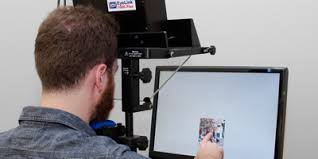
\includegraphics[width=.9\textwidth]{eye-tracker.jpeg}
			\pause
			\begin{itemize}
				\item Expensive
				\item Hard to analyse
			\end{itemize}
		\end{center}
	\end{column}\pause
	\begin{column}{.5\textwidth}
		\begin{center}
\textbf{\Large Self-paced reading}

\medskip

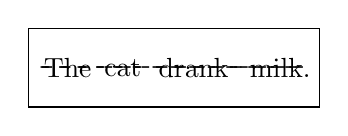
\begin{tikzpicture} %TODO on slide etc
\draw (-.5,-.5) rectangle (3.2,.5);
\onslide<4>{\node at (0,0) {The};}
\onslide<4>{\node at (1.7,0) {- - - - - - - - - - -};}
\onslide<5>{\node at (0,0) {- - - };}
\onslide<5>{\node at (.7,0) {cat};}
\onslide<5>{\node at (2,0) {- - - - - - - - };}
\onslide<6>{\node at (0.3,0) {- - - - - - };}
\onslide<6>{\node at (1.6,0) {drank};}
\onslide<6>{\node at (2.6,0) {- - - -};}
\onslide<7->{\node at (.9,0) {- - - - - - - - - - -};}
\onslide<7->{\node at (2.7,0) {milk.};}
\end{tikzpicture}
\end{center}
\onslide<8->{
			\begin{itemize}
	\item Lots of spillover
	\item Messy data 
\end{itemize}
}
\end{column}
\end{columns}
\end{frame}

\begin{frame}{A third option: Maze}
\end{frame}
\begin{frame}{Maze Task}
\centering
\tikzset{
	font={\fontsize{14pt}{12}\selectfont}}
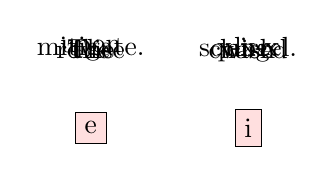
\begin{tikzpicture}
\onslide<1->{\node[draw] (a) at (-1,-.5) {e};}
\onslide<1->{\node[draw] (b) at (1,-.5) {i};}
\onslide<1-2>{\node  (c) at (-1,.5) {The};}
\onslide<1-2>{\node  (d) at (1,.5) {x-x-x};}
\onslide<3-4>{\node  (c) at (-1,.5) {upon};}
\onslide<3-4>{\node  (d) at (1,.5) {dog};}
\onslide<5-6>{\node  (c) at (-1,.5) {revise};}
\onslide<5-6>{\node  (d) at (1,.5) {chased};}
\onslide<7-8>{\node  (c) at (-1,.5) {the};}
\onslide<7-8>{\node  (d) at (1,.5) {wish};}
\onslide<9-10>{\node  (c) at (-1,.5) {mitigate.};}
\onslide<9-10>{\node  (d) at (1,.5) {squirrel.};}
\onslide<2,8>{\node[draw, fill=pink!50] at (a) {e};}
\onslide<4,6,10>{\node[draw, fill=pink!50] at (b) {i};}
\end{tikzpicture}
\end{frame}

\begin{frame}{A third option: Maze}
\begin{columns}
	\begin{column}{0.5\textwidth}
		\begin{center}
		\textbf{\large G-maze}
		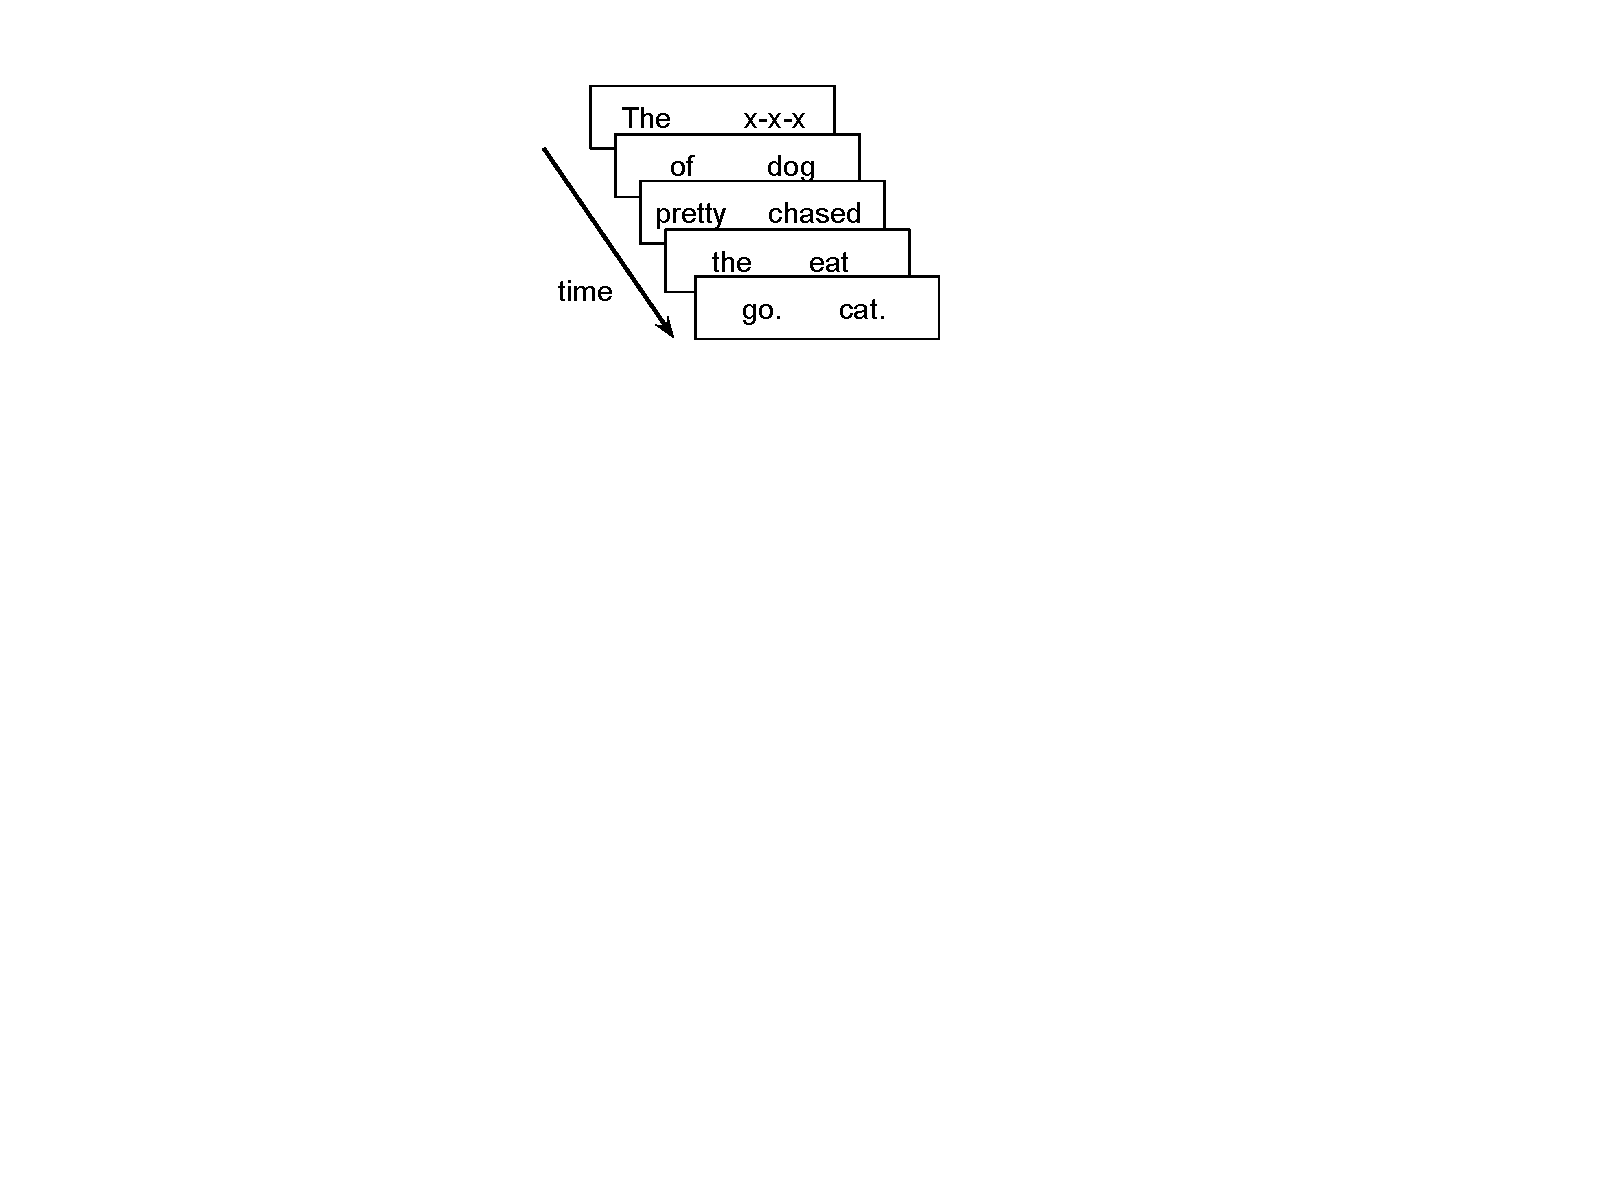
\includegraphics[clip, trim=9cm 14cm 11cm 1cm,width=.9\textwidth]{gmaze.pdf}
		\end{center}
	\pause
	\end{column}
	\begin{column}{0.5\textwidth} 
		\begin{center}
		\textbf{\large L-maze}
			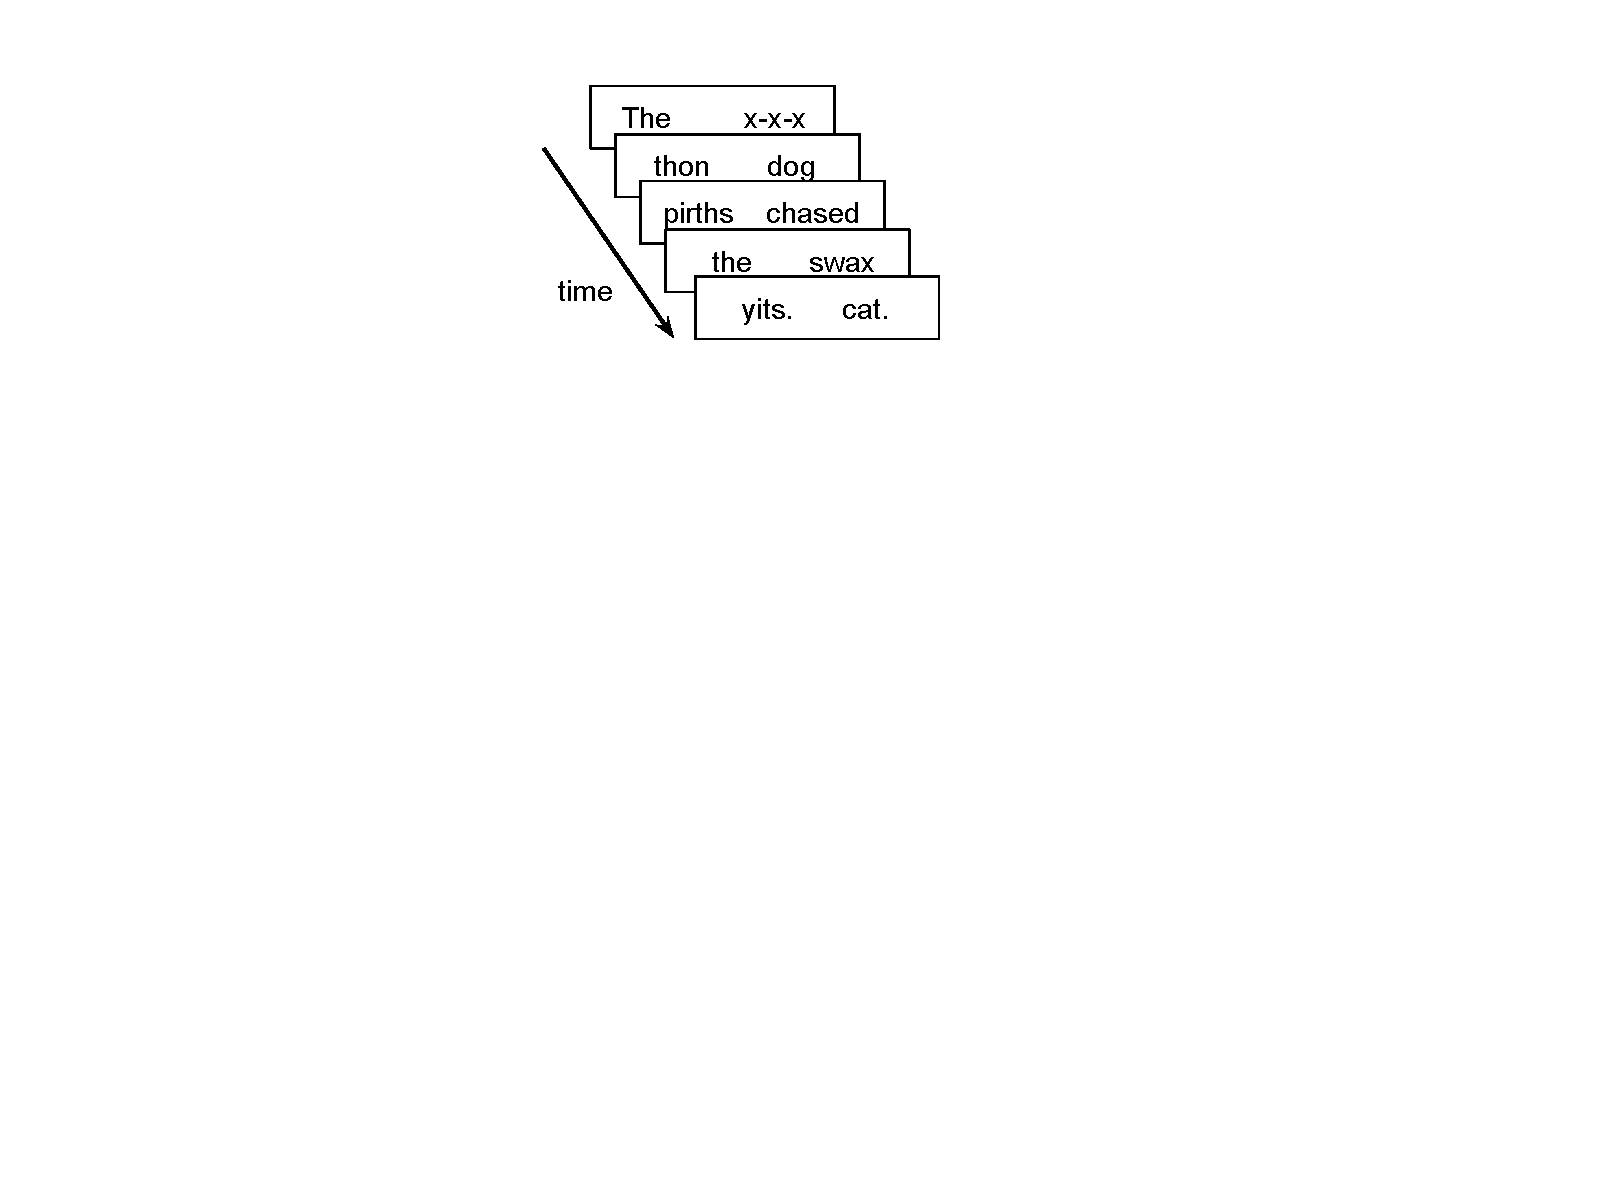
\includegraphics[clip, trim=9cm 14cm 11cm 1cm,width=.9\textwidth]{lmaze.pdf}
		\end{center}
	\end{column}
\end{columns}

\medskip
\pause
Sentence ends when a mistake is made.
\pause

Central claim: forces extremely incremental processing (no spillover)

\begin{flushright}
	{\small(Forster et al. 2009; Witzel et al. 2012)}
\end{flushright}
\end{frame}

\section{Experiment 1a}
\begin{frame}{Web Implementation}
Maze well suited to run on the web
\begin{itemize}
	\item Implement in Ibex
\end{itemize} 
\pause

Test by replicating Witzel et al. (2012)
\begin{itemize}
	\item Witzel et al (2012): Comparison of eye-tracking, SPR, L-maze, G-maze (all in-lab)
	\item Got materials and data from Witzel
	\item We run SPR, L-maze, and G-maze on MTurk
\end{itemize}
\end{frame}

\begin{frame}{Materials}

\textbf{Relative Clause}

\sethlcolor{green}
\textit{Low:} The son of the \uline{lady} who politely introduced \hl{herself} was popular at the party.
\sethlcolor{pink}

 \textit{High:} The \uline{son} of the lady who politely introduced \hl{himself} was popular at the party.
 

\textbf{Adverb Clause}

\sethlcolor{green}\textit{Low:} James will fix the car he \uline{drove} \hl{yesterday}, but he will need some help.

\sethlcolor{pink} \textit{High:} James \uline{will fix} the car he drove \hl{tomorrow}, but he will need some help.
		
\textbf{Sentence v Noun Phrase conjunction}

\sethlcolor{green} \textit{Comma:} The swimmer disappointed her \uline{coach}, and her mother \hl{tried} to console her.

\sethlcolor{pink}
\textit{No comma:} The swimmer disappointed her \uline{coach} and her mother \hl{tried} to console her.
\end{frame}

\begin{frame}{Results}
\begin{small}	
	\sethlcolor{green}
The son of the lady who politely introduced \hl{herself}\sethlcolor{pink} / \hl{himself} was popular at the party.
	
\end{small}
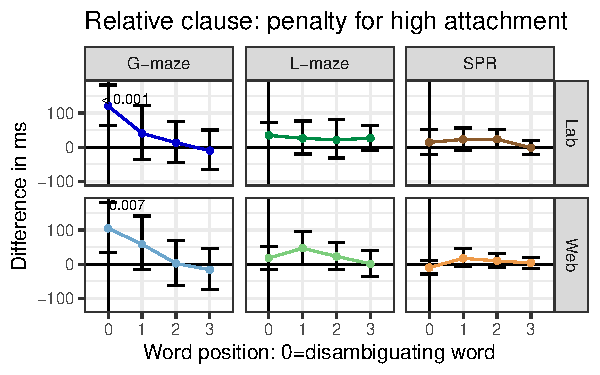
\includegraphics[width=\textwidth]{g_rel.pdf}
\end{frame}

\begin{frame}{Results}
\begin{small}	

\sethlcolor{green}James will fix the car he drove \hl{yesterday}\sethlcolor{pink} / \hl{tomorrow},  but he will need some help.

\end{small}
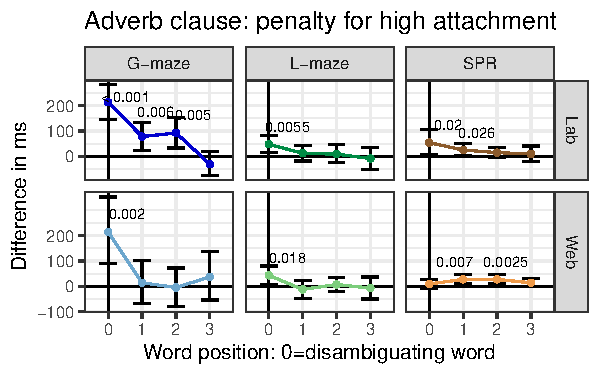
\includegraphics[width=\textwidth]{g_adv.pdf}
\end{frame}

\begin{frame}{Results}
\begin{small}	
\sethlcolor{green}The swimmer disappointed her coach\hl{,} and her mother \hl{tried} / \sethlcolor{pink}\hl{tried} to console her.
\end{small}
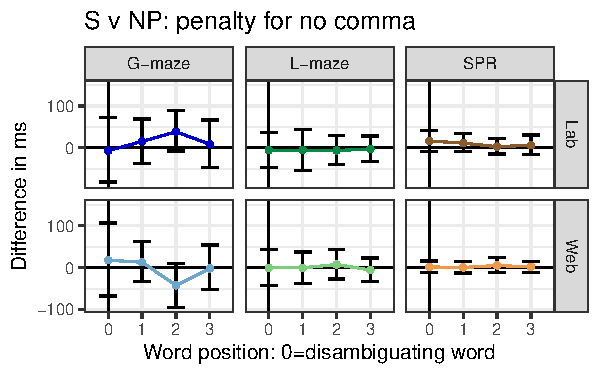
\includegraphics[width=\textwidth]{g_svnp.pdf}
\end{frame}

\begin{frame}{Interim Summary}
\textcolor{PineGreen}{\Large \textbf{Good news:} G-maze works well over the web (better than L-maze or SPR)}

\pause

\bigskip

\textcolor{Red}{\Large \textbf{Bad news:} I do not want to write G-maze materials.}


\end{frame}

\section{A-maze}

\begin{frame}{Meanwhile in Natural Language Processing}
\pause
Language models (LMs)
\begin{itemize}
	\item Trained on large corpora to predict the next word
	\item Given a partial sentence, return probabilities of the next word
\end{itemize}
\pause
Surprisal: negative log probability
\begin{itemize}
	\item 2 bits of surprisal = 1/4
	\item 10 bits of surprisal $\approx$ 1/1000 
	\item +1 surprisal = half as likely
\end{itemize}
\pause
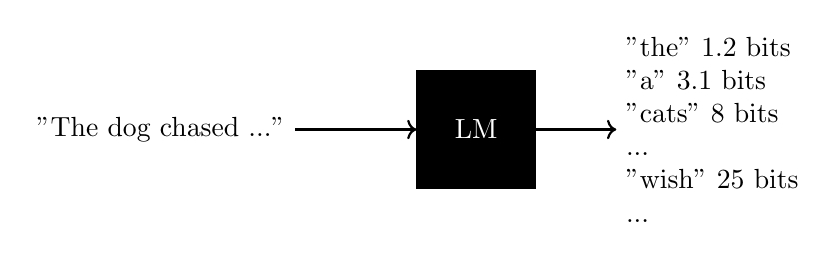
\begin{tikzpicture}
\node (A) at (0,0) {"The dog chased ..."};
\node  (B) at (4,0) [draw, minimum width=1.5cm, minimum height=1.5cm, fill=black] {\textcolor{white}{LM}} ;
\draw [->, thick] (A) -- (B); 
\node[align=left] (C) at (7,0) {"the" 1.2 bits \\"a" 3.1 bits\\"cats" 8 bits\\...\\"wish" 25 bits\\...};
\draw [->, thick] (B) -- (C); 
\end{tikzpicture}
\end{frame}

\begin{frame}{Can we use LMs to choose distractors?} 

Use high surprisal according to LM as a proxy for bad in context
\medskip

\pause

\begin{itemize}
	\item Model the target sentence word by word \pause
	\item At each position, choose a high surprisal word
\end{itemize}
\medskip
\pause
Want quality control on distractors
\pause
\begin{itemize}
	\item Restrict to a list of possible distractors \pause
	\item Only consider distractors of same length, frequency as target word \pause
	\item Check distractors until we find one with high surprisal \pause
\end{itemize}

\end{frame}

\begin{frame}
\centering
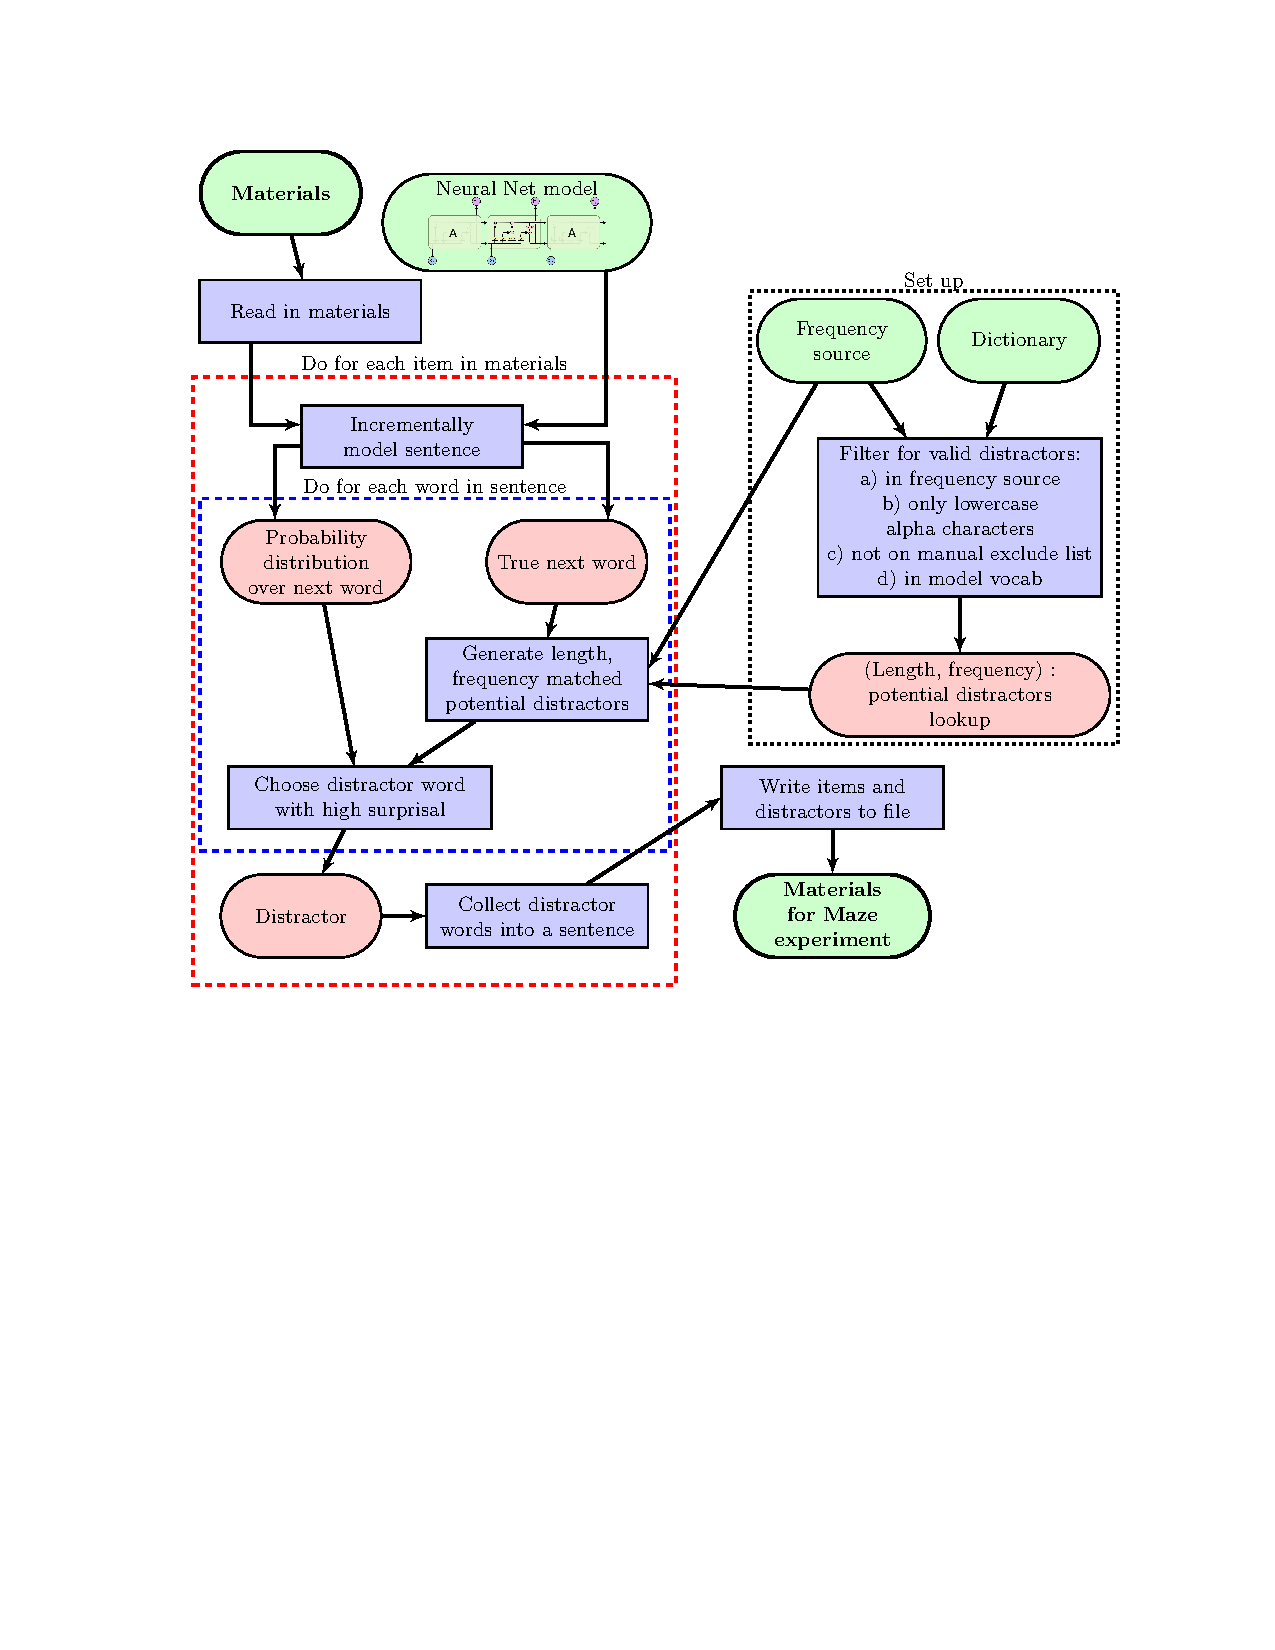
\includegraphics[clip, trim=3.25cm 5cm 2.5cm 2.5cm,width=.9\textwidth]{flow_2.pdf}
\end{frame}
\section{Experiment 1b}

\begin{frame}{Does A-maze work? }

Test it on materials from Witzel et al. (2012)
\medskip

Try with two pre-trained LSTM models (Gulordava 2018, Jozefowicz 2016)

\end{frame}

\begin{frame}{Does A-maze work?  Yes.} \pause
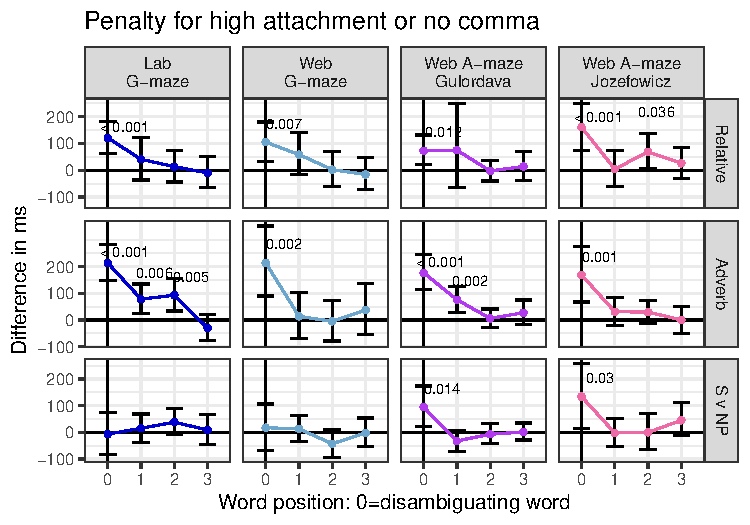
\includegraphics[width=1\textwidth]{a_all.pdf}
\end{frame}

\begin{frame}{Caveats}
A lot of mistakes on the second word of the sentence ("The \ul{dog} ...") \pause
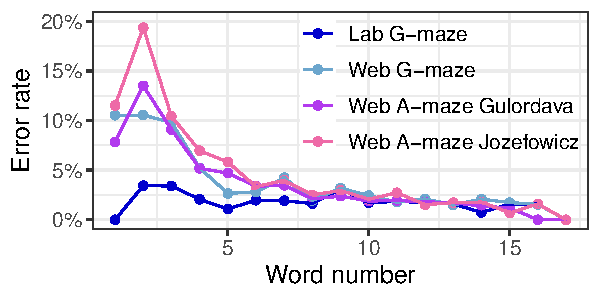
\includegraphics{../graph_errors2.pdf} \pause
Bad participants or bad distractors? 

Either way, lots of data loss.
\end{frame}

\begin{frame}{Caveats}

{\large Definitely some bad distractors}
\begin{table}
	
		
		\begin{tabular}{rlll}
			Prefix & Correct & Distractor & Error Rate \\
			\hline
			\hline
			Gulordava&&&\\
			\hline
			The & niece & cooks & 44\%\\
			The swimmer & disappointed & propositions & 30\%\\
			The & semester & steroids & 29\%\\
			\hline
			\hline
			 Jozefowicz&&&\\
			\hline
			The & husband & authors & 46\%\\
			Jim & listened & survived & 43\%\\
			The & uncle & roads & 42\%\\
			The & knight & saints & 40\%\\
		\end{tabular}
\end{table}

\end{frame}

\section{Experiment 2}

\begin{frame}{Potential improvements}

{\large Option 1: Choose better distractors.} \pause
\begin{itemize}
	\item Tweak thresholds of distractor selection. \pause
	\item Could search for optimal thresholds. \pause
	\item Could manually check and fix distractors. 
\end{itemize}

\end{frame}

\begin{frame}{Potential improvements}

{\large Option 2: Be forgiving.} \pause
\begin{itemize}
	\item Just don't terminate on mistakes. \pause
	\item Instead have participant correct mistake and continue.
	\end{itemize}
\end{frame}

\begin{frame}{Maze with Error Correction}
\centering
\tikzset{
	font={\fontsize{14pt}{12}\selectfont}}
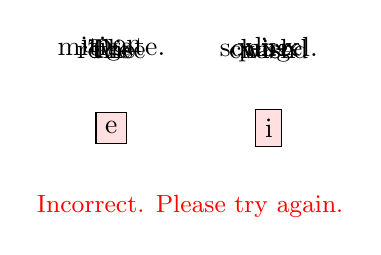
\begin{tikzpicture}
\onslide<1->{\node[draw] (a) at (-1,-.5) {e};}
\onslide<1->{\node[draw] (b) at (1,-.5) {i};}
\onslide<1-2>{\node  (c) at (-1,.5) {The};}
\onslide<1-2>{\node  (d) at (1,.5) {x-x-x};}
\onslide<3-4>{\node  (c) at (-1,.5) {upon};}
\onslide<3-4>{\node  (d) at (1,.5) {dog};}
\onslide<5-8>{\node  (c) at (-1,.5) {revise};}
\onslide<5-8>{\node  (d) at (1,.5) {chased};}
\onslide<9-10>{\node  (c) at (-1,.5) {the};}
\onslide<9-10>{\node  (d) at (1,.5) {wish};}
\onslide<11-12>{\node  (c) at (-1,.5) {mitigate.};}
\onslide<11-12>{\node  (d) at (1,.5) {squirrel.};}
\onslide<2,6,10>{\node[draw, fill=pink!50] at (a) {e};}
\onslide<4,8,12>{\node[draw, fill=pink!50] at (b) {i};}
\onslide<7,8>{\node[text=red] at (0,-1.5) {\small Incorrect. Please try again.};}
\end{tikzpicture}
\end{frame}

\begin{frame}{Maze with Error Correction}

{\large The ``solution'' to our problems!} \pause

\begin{columns}
	\begin{column}{0.3\textwidth}
		\begin{center}
		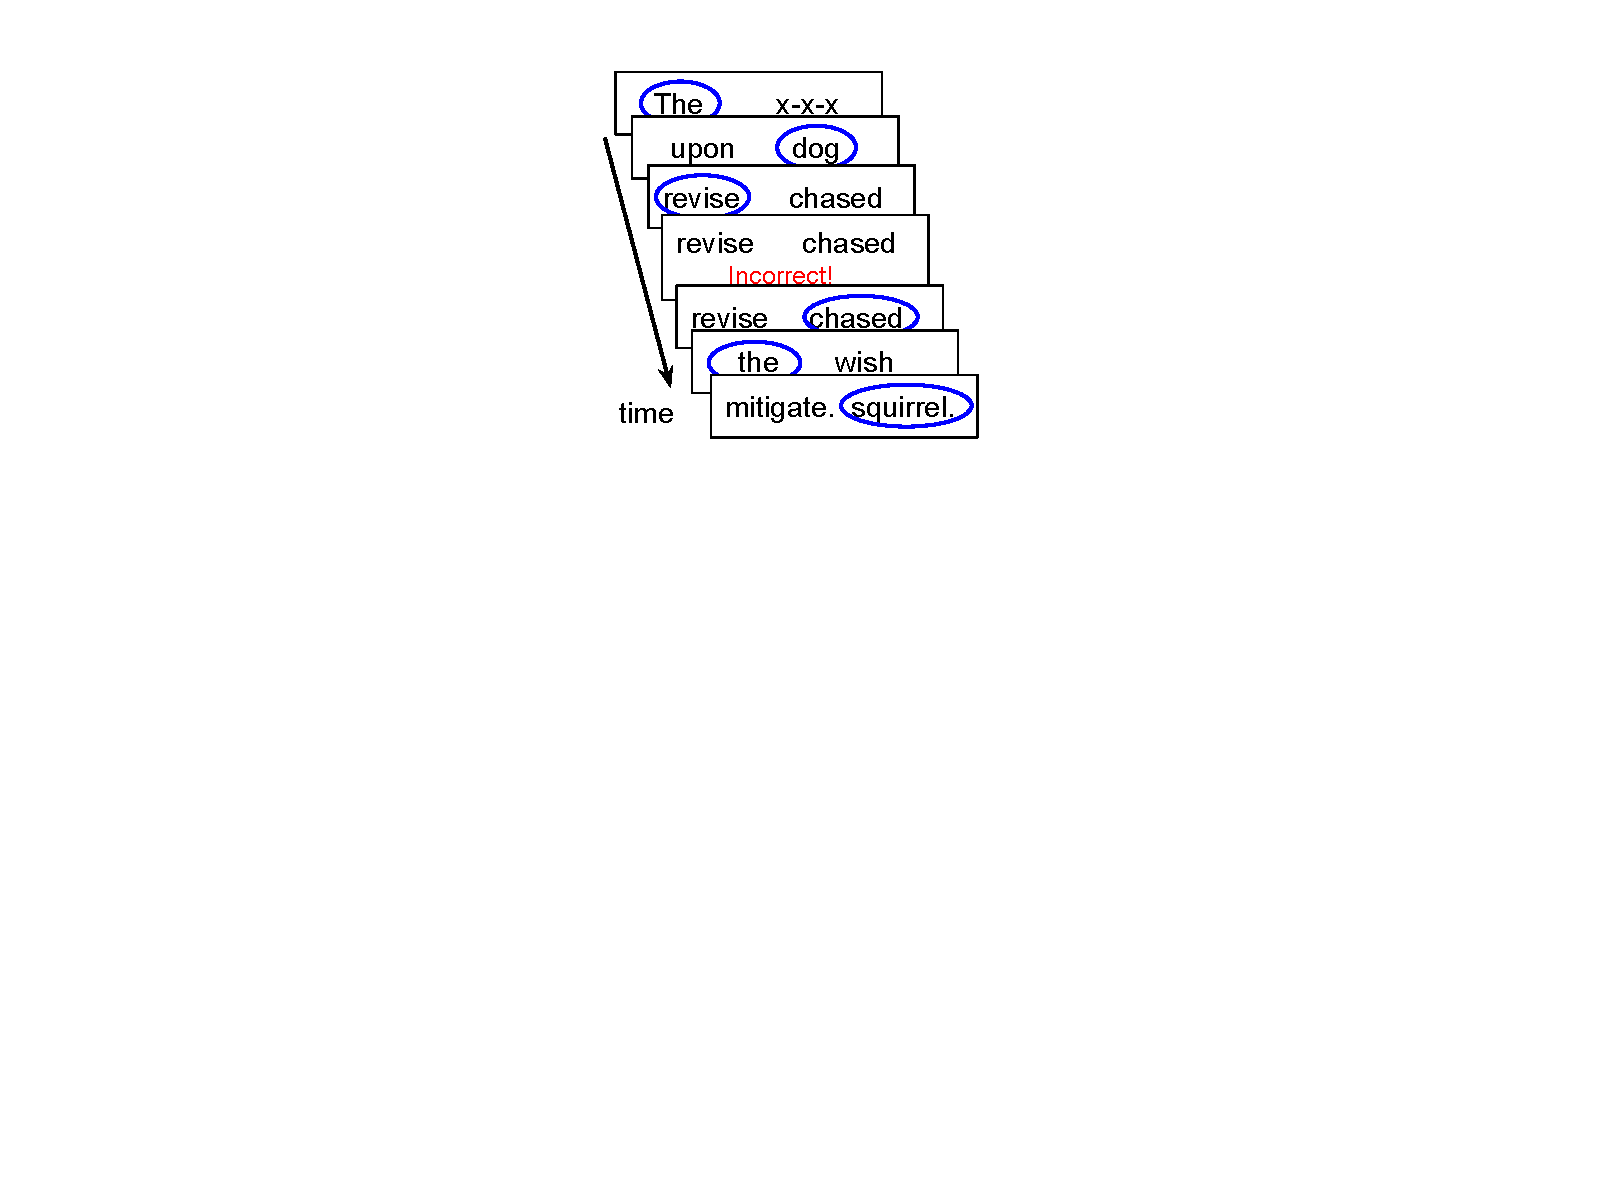
\includegraphics[clip, trim=9cm 12.5cm 10cm 1cm,width=\textwidth]{maze_diagram.pdf}
		\end{center}
		
	\end{column} \pause 
	\begin{column}{0.7\textwidth} 
		\begin{center}
			\begin{itemize}
				\item Easily implemented as a toggle in Ibex \pause
				\item Have all the data \pause
				\item Identify bad participants v bad distractors 
			\end{itemize}
		\end{center}
	\end{column}
\end{columns}
\medskip
\pause

Side effect: Can now run multi-sentence items!
\end{frame}

 %TODO: Needs work from here on!

\begin{frame}{Natural Stories}
Natural stories corpus (Futrell et al. 2017)
\begin{itemize}
	\item 10 stories, each about 1000 words
	\item Some unusual constructions, but read fluently
	\item 6 comprehension questions per story
\end{itemize}

\end{frame}

\begin{frame}{Natural Stories}

\begin{small}Tulip mania was a period in the Dutch Golden Age during which contract prices for bulbs of the recently introduced tulip reached extraordinarily high levels and then suddenly collapsed. At the peak of tulip mania in February sixteen thirty-seven, tulip contracts sold for more than ten times the annual income of a skilled craftsman. It is generally considered the first recorded economic bubble. [...]
\medskip

Q: When did tulip mania reach its peak?

A: \hspace{3em} 1630's\hspace{3em} 1730's \end{small}

\end{frame}

\begin{frame}{Experiment Plan}
Experiment questions:
\begin{itemize}
	\item Will people do this task?
	\item Can participants comprehend the stories?
\end{itemize}

\pause

\medskip
 
Checks on RT data
\begin{itemize}
	\item Check if RT is linear in surprisal (Smith \& Levy 2013)
	\item Check for known effects of word length, frequency
	\item Check for spillover effects
\end{itemize}

\end{frame}

\begin{frame}{Participant accuracy}
100 participants each read 1 story \pause
\begin{center}
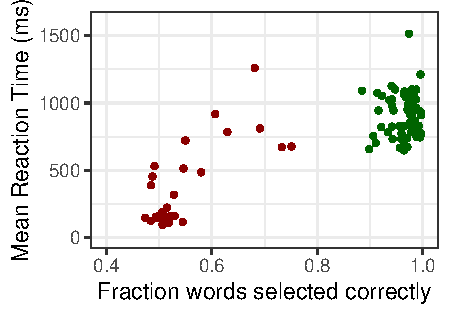
\includegraphics[width=.8\textwidth]{error.pdf}
\end{center}
\end{frame}
\begin{frame}{Comprehension questions}
\begin{center} \pause
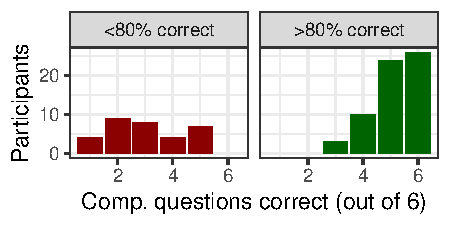
\includegraphics[width=.8\textwidth]{comp.pdf}
\end{center}
\end{frame}



\begin{frame}{Surprisal Effects}

Use 3 LMs to estimate surprisal: smoothed 5-gram, Gulordava RNN, Transformer-XL (Gulordava et al. 2018, Dai et al. 2019)
\pause

Fit GAMs on pre-error data.
\begin{itemize}
	\item Limit to single-token words.
	\item Fit to both current and past word surprisal.
\end{itemize}

\end{frame}

\begin{frame}{Surprisal Effects}
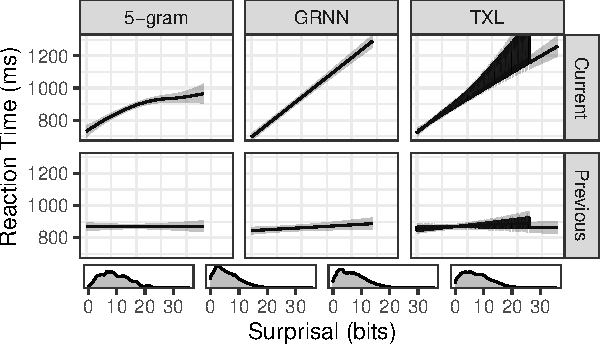
\includegraphics[width=.9\textwidth]{gam.pdf}	
\end{frame}
\begin{frame}{What about post-mistake data?}
Exclude data from mistakes or the two words after a mistake. 

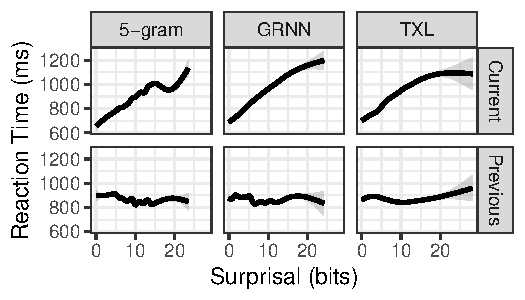
\includegraphics[width=.9\textwidth]{gam2.pdf}	
\end{frame}

\begin{frame}{Summary}
\begin{itemize}\pause
	\item People will read in the Maze task for 15-20 minutes \pause
	\item It's possible to comprehend during Maze \pause
	\item Distractors are generally good enough \pause
	\item Find expected RT patterns \pause
	\item Very little spillover
\end{itemize}
\end{frame}
\section{Conclusion}

\begin{frame}{Use A-maze!}
Easy to use! \pause
\begin{itemize}
	\item Runs on command line \pause
	\item Match distractors across minimal pair sentences \pause
	\item Customize surprisal thresholds, vocabulary lists \pause
	\item Can output pre-formatted for Ibex
\end{itemize}
\medskip
\pause
\end{frame}

\begin{frame}{Use A-maze!} \pause
Contribute to A-maze:
\begin{itemize}
	\item Written in Python 3 \pause
	\item Interface with other language models \pause
	\item Add more frequency sources \pause
	\item Extend to non-English languages
\end{itemize}

\end{frame}


\begin{frame}{}

\textcolor{ForestGreen}{\large Documentation: vboyce.github.io/Maze}

with links to the following:
\begin{itemize}

\item A-maze code: github.com/vboyce/Maze

\item Web-maze code: github.com/vboyce/Ibex-with-Maze

\item Sample task: syntaxgym.org:666

\item Paper: psyarxiv.com/b7nqd/
\end{itemize}
\end{frame}


\appendix

\begin{frame}{Matching distractors}
If unspecified: Match by position
\begin{itemize}
	\item The son of the lady who politely introduced \sethlcolor{green} \hl{herself}\sethlcolor{pink} / \hl{himself} was popular at the party.
\end{itemize}
Can specify labels for each word to pair (within item)
\begin{itemize}
	\item The cat who the dog scared hid in a box.\\pre-1 pre-2 who art noun verb main-verb post-1 post-2 post-3
\item The dog who scared the cat sniffed around the couch.\\ pre-1 pre-2 who verb art noun main-verb post-1 post-2 post-3
\end{itemize}
\end{frame}
%back pocket on more on model results??
%do we even need back pockets??

\begin{frame}{Post-mistake only}
Exclude data from mistakes or the two words after a mistake. 


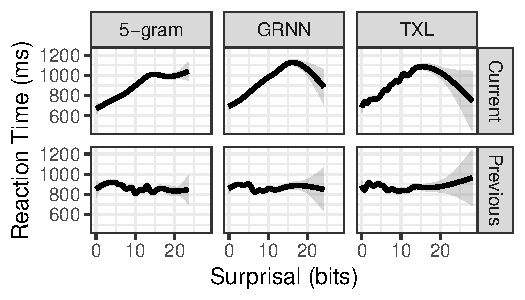
\includegraphics[]{gam3.pdf}	
\end{frame}


\end{document}

